%!TEX root = ./intern_report.tex

\newpage
\subsection{Designing and Implementing an Efficient End-toEnd Pipeline for Machine Learning in Robotics}

\begin{figure}[H]
    \centering
    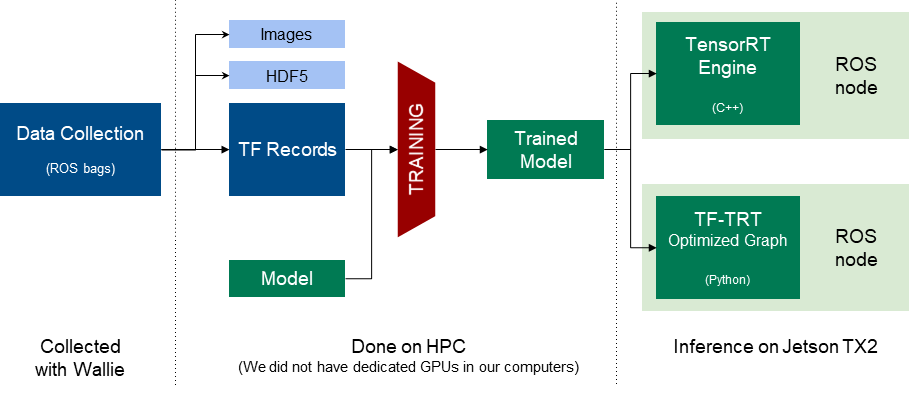
\includegraphics
        [width=16cm]
        {figures/full_pipeline.PNG}
    \caption{End-to-End Pipeline \label{Fig:pipeline}}\vspace{-4mm}
\end{figure}

\subsubsection{Training on Supercomputers}
\label{training_on_Supercomputers}

\subsubsection{TF Records}

\begin{figure}[H]
    \centering
    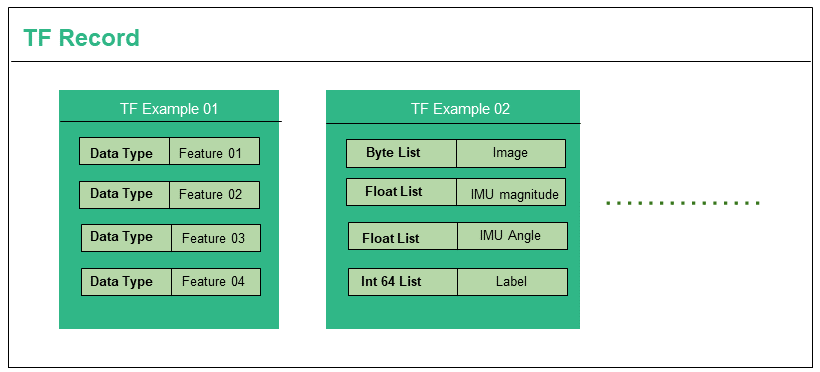
\includegraphics
        [width=9cm]
        {figures/tfrecord_structure.PNG}
    \caption{Structure of a TF Record}\vspace{-4mm}
\end{figure}

\begin{figure}[H]
    \centering
    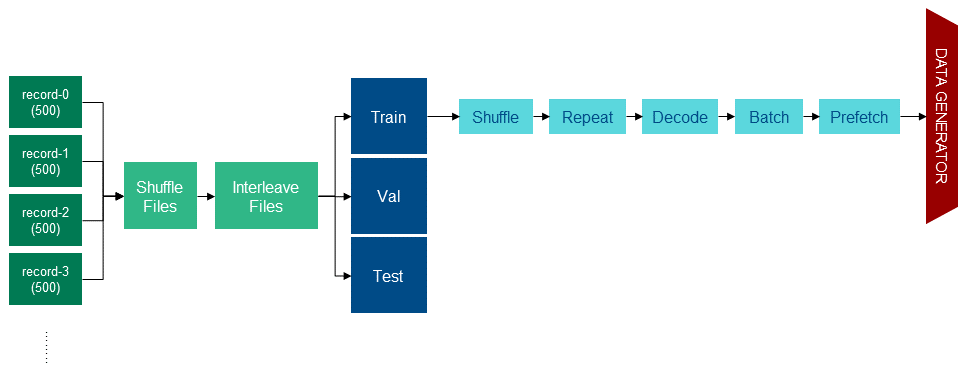
\includegraphics
        [width=16cm]
        {figures/input_pipeline.PNG}
    \caption{Data Input Pipeline with TFRecords}\vspace{-4mm}
\end{figure}


\subsubsection{TensorRT: Deployment on a low power device}
\label{tensorrt}

\begin{figure}[H]
    \centering
    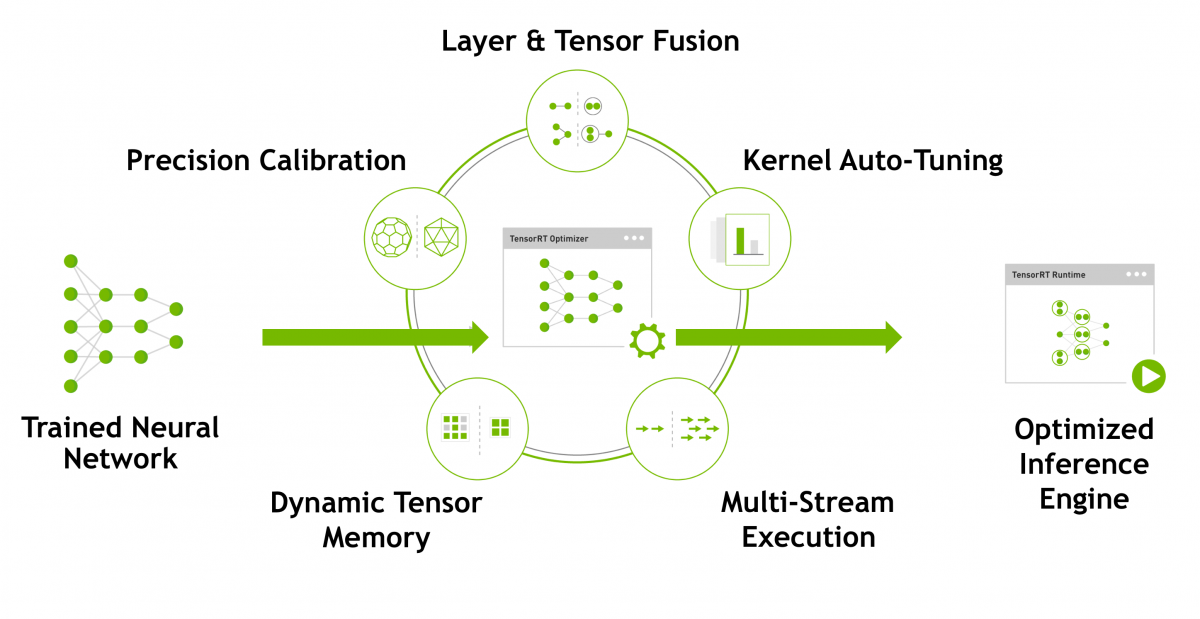
\includegraphics
        [width=13cm]
        {figures/trt.png}
    \caption{TensorRT in a nutshell}\vspace{-4mm}
\end{figure}

\begin{figure}[H]
    \centering
    
\includegraphics
        [width=13cm]
        {figures/deploy_pipeline_cpp.PNG}
    \caption{Deployment Pipeline: C++}\vspace{-4mm}
\end{figure}

\begin{figure}[H]
    \centering
    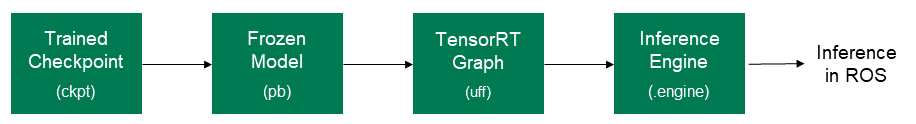
\includegraphics
        [width=13cm]
        {figures/deploy_pipeline_python.PNG}
    \caption{Deployment Pipeline: Python}\vspace{-4mm}
\end{figure}

\subsubsection{Problems Faced and Solutions}